\chapter{Testing}
\label{chapter:testing}

Testing is a crucial task to ensure that the application functions now and in the future, according to the given requirements.
Even though testing doesn't ensure bug free code, it reduces the number of (unnoticed) bugs, and the chance of errors.
It also does not protect against logical errors or oversights.
I tested both the frontend and backend applications exhaustively.
The proxy application I opted not to test, as it is mostly a lightweight wrapper around the Kubernetes JavaScript client library, which itself is already well-tested by its creators and maintainers.

\section{Backend}
\subsection{Setup}
The backend is written primarily using the Laravel PHP web framework as stated beforehand.
As the first step the application has to be installed and set up.
This can be done with Laravel's own installer, where many application templates can be selected.
A React template is available, however that uses Inertia.JS by default which is a package that enables the frontend to be server side routed a minimal API backend template.
So Laravel will serve as an API backend and the view layer of the MVC architecture will be entirely handled by the frontend.

After installation, I decided to install the Laravel Sail package which provides a preconfigured development Docker Compose setup, and also provides options to install additional components into our environment.
The extra containers in our case will be the MySQL database, the Mailpit SMTP test server and the MinIO S3 compatible object storage.
Sail is however published as a package which by default would need a local PHP and Composer (PHP's package manager) installation.
This would kind of defeat its purpose.
Luckily this can be avoided by using a temporary PHP container to quickly install initial dependencies and then use the Sail application for further required packages.

Afterwards the provided \texttt{.env.example} file needs to be copied to \texttt{.env} and the appropriate environment variables need to be set, including the mail server, database and object storage connections.
Finally, the application key must be initialized using the Artisan CLI and the default database migrations have to be run.

\subsection{Data Layer}

Let me start building up the backend's feature set from the bottom, starting with the parts of the Eloquent ORM.
The database schema of the backend including the most important tables can be seen on Figure \ref{fig:database}.

\textit{Note:} Laravel has some other default tables, related to built-in features such as jobs and caching that I omitted from the diagram for better clarity as they will be unused in the application.

\begin{figure}[H]
  \centering
  \includegraphics[width=\linewidth]{./figures/database.png}
  \caption{Database schema}
  \label{fig:database}
\end{figure}

The 'users' table is auto generated, the only change I made is regarding the ID (Identifier) field.
In all tables and models I opted to switch from the default integer ID to UUIDv7 (Universally Unique Identifiers version 7) which are time-based sortable universally unique identifiers composed of 32 hexadecimal digits.

The role related tables are added by the Spatie's Laravel Permission package, which I will talk about in more detail in the authorization Subsection \ref{subsection:authorization}.

On the other hand the media table is added by

\subsection{Authentication}
\subsection{Authorization}
\label{subsection:authorization}
\subsection{Core CRUD}
\subsection{Deployment Logic}
%TODO: Sequence diagram for deployment logic?
\subsection{Admin Panel}
\chapter{Frontend}
\label{chapter:frontend}
\section{Setup and overview}
\label{section:frontend-setup}
I implemented the frontend using React first and foremost.
The most important packages I used are TanStack Router for client side routing, TanStack query for robust data fetching and caching, and CraftJS for the editor capabilities.

As the first step, the React app has to be installed.
I scaffolded the application using the Vite bundling tool's CLI and chose a TypeScript based application.
Then I set TypeScript to use strict type checking to disallow \texttt{any} types, and also installed TailwindCSS and its Vite plugin as I used the ShadCN UI components.
ShadCN distributes its components and blocks in an open code manner through the npx CLI, which means that instead of installing a npm package, the source code of the block gets copied into the application.
This has the advantage that the components can be completely customized if needed, and the downside that the repository size grows considerably.

I also used predesigned UI blocks form ShadCN.IO \cite{shadcn.io_2025}.
While I was building the application all components from this site were open-sourced and free, however as of writing this documentation they introduced many new blocks that got locked behind a subscription. Previously free blocks remained as such, but require a free account now. This change doesn't affect the application as the source code got inserted into the project directly so further use and modification is possible.

Next I used Docker's init command to scaffold a Dockerfile and docker-compose.yaml for containerization, to which I only made minor changes, mostly regarding setting up environment variables.
I also configured ESLint, which is a static code analyser, to ensure better code quality.

Since unlike Laravel, React is unopinionated about the structure of the application, let me talk about how I architected the frontend's folder structure.
I was partly inspired by the Bulletproof React repository \cite{alan2207/bulletproof-react}, however I made a few changes to better fit my needs.
The high level overview of the layout can be seen on Figure \ref{fig:react-structure}.

\begin{figure}[H]
  \centering
  \includegraphics[width=\linewidth]{./figures/frontend-struct.png}
  \caption{React application structure}
  \label{fig:react-structure}
\end{figure}

The \texttt{main.tsx} is the setup file for the frontend application, about which I will go into detail shortly.
The \texttt{routeTree.gen.ts} contains the routing tree that TanStack router generates.
For more information about this refer to Subsection \ref{subsection:tanstack-router}.
The \texttt{components} folder contains the UI elements added by the ShadCN library and other component blocks I created using them that are global to the application.
The \texttt{context} includes the globally defined application contexts, that I will talk about in Section \ref{section:api-context}.
Inside \texttt{hooks} live the custom React hooks that I defined.
\texttt{Lib} collects utility functions, global constants and the generated API client, which I will elaborate in Section \ref{section:api-context}.
The \texttt{providers} folder houses the context providers that the aforementioned context objects return.
\texttt{Routes} encompass not only the route hierarchy but using the router's \texttt{-} notation it also colocates any route specific components and logic.
The \texttt{testing} folder accommodates all test related files.
Refer to Section \ref{section:testing-frontend} for a thorough explanation.
Finally, \texttt{types} include all TypeScript types that are either generated by the API client or Zod schemas.

Zod is a library used for schema validation primarily focusing on TypeScript.
I used it in conjunction with React Hook Form, a hook based form library for React, to generate form schemas and provide client side validation.
I also validated search parameters using it in a few routes. A great feature of Zod is that TypeScript types can be inferred from form schemas for further use.

Now let me talk about setting up the application in the \texttt{main.tsx} file.
Some details will be expanded upon later but are understandable at this point as well.

First a router instance has to be constructed, to which the route tree needs to be provided. Additionally, the router context has to be configured with initial values.
This has to include everything that routes need to have access to before even rendering their component.
In my case this contained TanStack query's query client, which is constructed here, the auth context, and a default callback that returns the given routes title.
The latter will be overridden in each route and will be used for breadcrumb generation.
The auth context is undefined at this point and will be updated later.
Here I also set up a default view transition that provides a smoother animation between route switching and scroll restoration.
Moreover, I configured the loader stale time to 0 (never stale) as the query client will handle that instead of the router (both share this concept).
Finally, I changed the default preload method to 'intent', which has the effect of launching loader preloads after 50 milliseconds when a user hovers on the link of the destination route.

Next a component I called \texttt{InnerApp} has to be created.
This component's only purpose is to have access to the useAuth hook and return the router provider with the router instance and a now existing valid authentication context.
The router provider will take care of rendering child routes.

Moving on, I created an \texttt{App} component which wraps the previous \texttt{InnerApp} with the auth provider, the theme provider, and query client provider.
The query client provider has access to the same query client as the router.
Also, I included the \texttt{Toaster} component from the Sonner package created by Emil Kowalski alongside the \texttt{InnerApp}.
This package an easy-to-use and opinionated way of making toast notifications.
I primarily use it to provide feedback to the user from background tasks such as API calls.

Last but not least the \texttt{App} itself is surrounded with React's strict mode component that enables development only extra behaviours with the aim of finding common bugs.
In production, it has no effect and is turned off.
At the end of all this, the component chain gets rendered by the root React DOM object, which finishes the setup process, as the \texttt{index.html} by default includes the \texttt{main.tsx} script.

One last thing I want to talk about here is the root route.
It must be named as \texttt{\_\_root.tsx} and is the root of the route tree. Here the library's Outlet component has to be returned which will take care of rendering all child routes.
Additionally, I implemented application wide, loading, not found and error boundary components to provide a better UX for these scenarios.

For example Figure \ref{fig:not-found} the not found component that renders when a user navigates to a non-existent route.

\begin{figure}[H]
  \centering
  \includegraphics[width=\linewidth]{./figures/not-found.png}
  \caption{Not found component for missing routes}
  \label{fig:not-found}
\end{figure}
\section{API client and context providers}
\label{section:api-context}

After the setup process, I will move on to describing the features mainly in the \texttt{context}, \texttt{providers}, \texttt{hooks}, and \texttt{lib} folders.

Generating the OpenAPI schema of the backend has the great benefit of allowing me to take advantage of the many available libraries specializing in API client code generation.
I investigated a couple of existing solutions, namely Orval, Kubb, and OpenAPI-TS.
Orval and Kubb both feature an extendible approach where you can pick what you want to use.
However, they both proved to be way more complicated than what I needed, so I opted to use OpenAPI-TS.
OpenAPI-TS provides many smaller libraries that provide client-side code generation from OpenAPI schemas.
For my use case OpenAPI-React-Query was the one I needed and ended up using.
It is a tiny, around 1kb wrapper around TanStack Query and incorporates two other libraries by the same author, OpenAPI-Fetch and OpenAPI-TypeScript.
It validates the available API routes inside the query calls, checks parameters and bodies, and can be used to generate TypeScript types for the requests and responses.

Next I generated the API client with the library in the \texttt{lib/api} folder and also customized the fetch client used by it.
Namely, I created a custom \texttt{APIError} class that handles error messages from the backend, configured the base URL from environment variables and the default headers.
Additionally, since the backend uses CORS and CSRF protection it requires requests to have a valid XRSF token.
This can be obtained by first making a request to the \texttt{/sanctum/csrf-cookie} endpoint.
This was also configured in the fetch client to be handled automatically and re-fetch when the token expires.

Moving on, I implemented the custom theme and authentication providers.
I was guided by the ShadCN documentation \cite{shadcn_2025} on how to configure light, dark, and system themes using TailwindCSS's functionality.
The provider stores the selected theme in and recovers it from the browser's local storage on subsequent visits.
Toggling the themes are possible from the account page, and the app defaults to the system theme.
Accessing the theme in other components is possible through a custom \texttt{useTheme} hook.

Afterwards I created the authentication provider for auth state management.
It provides through the \texttt{useAuth} hook methods for logging in, registering, logging out, re-fetching user context and deleting the account.
All these methods use the API client wrapping TanStack Query's mutations and query functions.
The context encompasses two React states, one a boolean for quick checks, and the other containing the logged-in user's information.
I also store the state in the browser's local storage and recovered upon mounting by an \texttt{useEffect} call so that the user remains logged in on revisits.
\section{Authentication, dashboard, and account routes}

In this block, I will mainly be presenting the authentication and account related pages that I created on the frontend.
To begin with, a use case diagram in Figure \ref{fig:auth-use-case} shows in detail the authentication capabilities.

\begin{figure}[H]
  \centering
  \includegraphics[width=\linewidth]{./figures/auth-use-case.png}
  \caption{Authentication use cases}
  \label{fig:auth-use-case}
\end{figure}

Guests or unauthenticated users can log in, register, and ask for a forgot password link, which redirects them to a form allowing them to reset their password.
Authenticated users can verify their emails, which they automatically get an email for after registration, or can request a new one on the account page, which I will talk about later.
Obviously, if the user clicks on the verification link in their email while being unauthenticated they will first be redirected to the login page.

When a user first visits the frontend, a simple index page greets them with directions to login, or register, or go to the dashboard if they are already logged in.
The index page as shown for an unauthenticated user can be seen in Figure \ref{fig:index-page}.

\begin{figure}[H]
  \centering
  \includegraphics[width=\linewidth]{./figures/index-page.png}
  \caption{Index page for an unauthenticated user}
  \label{fig:index-page}
\end{figure}

From the landing page, the user can directly log in and/or register.
As stated previously, I used React Hook Form with Zod for creating all my forms.
This ensures that there is proper client side validation, and can be used to display meaningful error messages to the user.
All forms also employ a loading state to prevent multiple submissions while a previous request is running.
I also display success and error responses using the aforementioned toast notifications in the bottom right corner of the screen.
The registration page with an example for validation errors can be seen in Figure \ref{fig:register}.

\begin{figure}[H]
  \centering
  \includegraphics[width=\linewidth]{./figures/register.png}
  \caption{Register page with validation errors}
  \label{fig:register}
\end{figure}

The rest of the forms look almost identical to the registration one, so I won't show each of them one-by-one unnecessarily.
One thing worth mentioning is that both the registration and forgot password links send out emails.
Such an example email after registration captured by Mailpit can be seen in Figure \ref{fig:email}. On the sidebar the incoming password reset links can be seen as well.

\begin{figure}[H]
  \centering
  \includegraphics[width=\linewidth]{./figures/email.png}
  \caption{Registration email seen in Mailpit}
  \label{fig:email}
\end{figure}

After logging in, the user can access the main application routes grouped by the \texttt{\_app} folder.
They are all surrounded with a layout component that has two main responsibilities.
First, check if the user has successfully logged in, if not, redirect them to the login route.
Secondly, this is where the title callback I mentioned in Section \ref{section:frontend-setup} is used.
The layout component collects the result of all title callbacks from the router state, which include the title names for all rendered child routes.
Afterwards, it dynamically builds the breadcrumb trail displayed to the user.

The first such route is the dashboard, which displays a few statistics and quick actions.
Figure \ref{fig:dashboard} showcases it in detail.

\begin{figure}[H]
  \centering
  \includegraphics[width=\linewidth]{./figures/dashboard.png}
  \caption{The dashboard page}
  \label{fig:dashboard}
\end{figure}

Next, let me provide and overview of account settings, which can be accessed via a pop-over by clicking on the user section of the sidebar.
Another use case diagram showcasing the account-related options can be seen in Figure \ref{fig:account-use-case}.

\begin{figure}[H]
  \centering
  \includegraphics[width=\linewidth]{./figures/account-use-case.png}
  \caption{Account settings use cases}
  \label{fig:account-use-case}
\end{figure}

The user is able to switch the application between light, dark, and system themes.
They can also update their profile information, which includes changing their display name and email.
Changing the email automatically sends a verification email to the new address.
They can upload an avatar via a drag and drop field or the system file picker, which can be previewed before saving.
A tab, which shows the verification status is available, and if unverified, a new link can be sent from here.
Passwords can be changed using a form that shows the new password's strength using simple metrics like length and contained special characters.
After changing it, the user will be logged out automatically and prompted to log in again.
Lastly, the account can be deleted if the user wishes so.
This will first show a confirmation dialog to avoid accidental deletion.

Two pictures comparing light and dark modes can be seen in Figure \ref{fig:theming}.
The light mode picture on Subfigure \ref{subfig:light-avatar} showcases the avatar upload tab, while the dark mode picture on Subfigure \ref{subfig:dark-password} presents the password change form.
The light mode picture also displays how to get to the account settings page.

\begin{figure}[H]
  \centering
  \begin{subfigure}[b]{0.49\textwidth}
    \centering
    \includegraphics[width=\textwidth]{./figures/light-avatar.png}
    \caption{Light mode avatar upload}
    \label{subfig:light-avatar}
  \end{subfigure}
  \hfill
  \begin{subfigure}[b]{0.49\textwidth}
    \centering
    \includegraphics[width=\textwidth]{./figures/dark-password.png}
    \caption{Dark mode password change}
    \label{subfig:dark-password}
  \end{subfigure}
  \caption{Dark and light modes}
  \label{fig:theming}
\end{figure}
\section{Schemas, sites, and pages}

Next up, let me talk about creating and managing schemas.
As with the previous features, I present a use-case diagram of them in Figure \ref{fig:schema-use-cases}.

\begin{figure}[H]
  \centering
  \includegraphics[width=\linewidth]{./figures/schema-use-cases.png}
  \caption{Schema use cases}
  \label{fig:schema-use-cases}
\end{figure}

Schemas can be used as templates for pages, which I will mention the details of later.
Most of the use cases include basic CRUD operations.
Users, however, have to have a verified email to access schemas (sites and pages too), and also they can only view them. They also only see published schemas.
Only administrators are capable of editing, designing, and publishing schemas for users to reuse.
I used similar page designs for related features across schemas, pages, and sites, so I won't show each page related to the schemas here.
In Figure \ref{fig:schema-list} a list view of schemas can be seen.

\begin{figure}[H]
  \centering
  \includegraphics[width=\linewidth]{./figures/schema-list.png}
  \caption{Card list of schemas}
  \label{fig:schema-list}
\end{figure}

At the bottom of the screen, the pagination component is visible, and the hovered first card has a shadow and shading applied.
The detailed view of schemas is almost identical to the pages.
For an idea on how that looks, see Figure \ref{fig:page-detail}.
The schema edit and create page is basically the same, and it is a simple form that can be viewed in Figure \ref{fig:schema-edit}.

\begin{figure}[H]
  \centering
  \includegraphics[width=\linewidth]{./figures/schema-edit.png}
  \caption{Schema edit form}
  \label{fig:schema-edit}
\end{figure}

The designer for schemas is the same as the one for the pages and is the main topic of Section \ref{section:editor}.

The next resource on the frontend is the sites.
Once again, a use case diagram of site related features is visible in Figure \ref{fig:site-use-cases}.

\begin{figure}[H]
  \centering
  \includegraphics[width=\linewidth]{./figures/site-use-cases.png}
  \caption{Site use cases}
  \label{fig:site-use-cases}
\end{figure}

Sites encompass their pages. They have a two tabbed detail view, one showing general information, while the other shows their pages.
It also contains controls for deploying the application if it has not been published yet.
If it has, it is possible to restart, update and delete it from the dropdown.
A confirmation dialog appears in all mentioned cases.
The detail view of the site appears in Figure \ref{fig:site-detail}.
Subfigure \ref{subfig:site-overview} shows the general information, deployment controls, buttons that take the user to the edit form and designer pages, and a delete button for deleting the site and all its resources.
A toast notification indicating a successful restart is also visible.
On the other hand, Subfigure \ref{subfig:site-pages} shows the pages of the site where their detail view can be visited by clicking on a card, or a new one can be created with the provided button.

\begin{figure}[H]
  \centering
  \begin{subfigure}[b]{0.49\textwidth}
    \centering
    \includegraphics[width=\textwidth]{./figures/site-restart.png}
    \caption{Overview tab}
    \label{subfig:site-overview}
  \end{subfigure}
  \hfill
  \begin{subfigure}[b]{0.49\textwidth}
    \centering
    \includegraphics[width=\textwidth]{./figures/site-pages.png}
    \caption{Pages tab}
    \label{subfig:site-pages}
  \end{subfigure}
  \caption{Site detail view}
  \label{fig:site-detail}
\end{figure}

Regarding the deployment options, this and the schema publish is the only scenario in the frontend where I have to use manual query invalidation to update the displayed data in time.
This is because we stay on the same view, instead of navigating away, which would normally trigger SWR's re-fetch mechanism.
All three resources I talk about in this section also have an empty component that is displayed if the returned API answer is an empty collection.
Figure \ref{fig:site-empty} displays the one belonging to sites.

\begin{figure}[H]
  \centering
  \includegraphics[width=\linewidth]{./figures/site-empty.png}
  \caption{Site's empty component}
  \label{fig:site-empty}
\end{figure}

Finally, let me talk about the pages. As with the previous two cases, Figure \ref{fig:page-use-cases} shows a use case diagram for existing page related actions.

\begin{figure}[H]
  \centering
  \includegraphics[width=\linewidth]{./figures/page-use-cases.png}
  \caption{Page use cases}
  \label{fig:page-use-cases}
\end{figure}

The editor related actions, such as generating the HTML content, play core parts in saving the page to the backend.
Most other functions are identical to schemas and sites.
A crucial difference is the creation form.
Since pages can be based off of schemas, the creation form needs to be able to provide the ability to select a schema as the base content for a page.
Later, this of course can be edited by the user without it having any effect on the original schema.
The form basically copies its content into the page.
To solve this problem, I created a multistep form using the Stepperize React library, which has built-in support for the ShadCN UI components \cite{stepperize_2025}.
Figure \ref{fig:page-create} showcases this form and the schema selection step. Schemas can be previewed here via a dialog.

\begin{figure}[H]
  \centering
  \includegraphics[width=\linewidth]{./figures/page-create.png}
  \caption{Page creation multistep form}
  \label{fig:page-create}
\end{figure}

At the end of the form I show the user a review tab, and the process can also be reset here if needed.
The page edit form is similar to the schema edit form in Figure \ref{fig:schema-edit}.
The detail view of the pages also contains a preview of the content for easier identification.
Figure \ref{fig:page-detail} presents this functionality.

\begin{figure}[H]
  \centering
  \includegraphics[width=\linewidth]{./figures/page-detail.png}
  \caption{Page details with content preview}
  \label{fig:page-detail}
\end{figure}
\section{Editor}
\label{section:editor}

The editor or designer is undeniably the most complex and central component of the frontend.
It uses the CraftJS library for its core functionalities.
I reused this component in both schemas and pages, by passing a callback from the parent component that handles the saving functionality, which is the only difference it this case between the two.

CraftJS allows the developer to define editable components.
It leverages this by providing custom React hooks.
These define the editable props, what options can be set for these props, whether the component is editable or not, and what regions can the user drop specific components to inside itself.

The full use cases of the developed designer can be viewed in Figure \ref{fig:designer-use-cases}.

\begin{figure}[H]
  \centering
  \includegraphics[width=\linewidth]{./figures/designer-use-cases.png}
  \caption{Use cases of the designer component}
  \label{fig:designer-use-cases}
\end{figure}

The editor with some example components inserted is displayed in Figure \ref{fig:editor-base}.

\begin{figure}[H]
  \centering
  \includegraphics[width=\linewidth]{./figures/editor-base.png}
  \caption{The editor filled with example content}
  \label{fig:editor-base}
\end{figure}

I composed the designer of three main components.
The first and most important is the editor area, which shows the design the user is creating.
This is a resizeable canvas to which users can drag and drop the editor's components.
On hovering over the components, an outline appears for the selection, showing the name of the component, a mover icon prompting that it can be moved, and a delete button to remove it from the page.
When dragging components around, green and red lines show that the given component can or cannot be moved to the new desired location.

The second is the top bar, which contains the control buttons.
On the left side is a toggle that enables or disables preview mode.
The preview mode prevents any sort of edits and changes, and the sidebar of the editor, which is the third main component I will mention shortly, reflects this as well.
Next to this is the buttons for undoing and redoing changes, for which I also implemented the usual keyboard shortcuts.
CraftJS provides this functionality natively by itself, through a hook.

The middle section of the top bar has viewport controls that resize the editable area to see how the page would look like on desktop (default), tablet and mobile sized screens.
There is also a button to view the content in full screen, from which exiting is also possible by pressing the Escape key.
Lastly, in this area I placed a reset button to exit full screen and or return the viewport to the desktop size.

Figure \ref{fig:editor-preview} showcases the designer in preview and full screen mode.

\begin{figure}[H]
  \centering
  \includegraphics[width=\linewidth]{./figures/editor-preview.png}
  \caption{Editor full screen preview}
  \label{fig:editor-preview}
\end{figure}

The third section of the top bar houses a copy button for quick copying of the editor content, and a load button that allows rebuilding the page from the copied content through a dialog.
Lastly, I located the save button for saving the changes to the database here.
Related to saving, I also implemented navigation blocking for pages that use this component.
This displays the built-in alert of the browser notifying the user that unsaved changes will be lost upon leaving the page.

Before I describe the editor sidebar, I briefly want to talk about saving the content.
CraftJS serializes the editor content into a JSON structure describing the component tree of the edited page.
The root component is the canvas to which components can be dropped to.
Each node of this tree also describes the props of the component and what values users passed to it.
It is easy to see that this tree can grow large relatively quickly.
Due to this, I used the Pako library providing a zlib port to JavaScript, to compress the JSON tree \cite{nodeca/pako}.
I then also base64 encoded this to further reduce its size for network transfer.
The steps described above, however, only take care of the JSON, but the static HTML has to be somehow generated as well.
To achieve this, I create an empty div to which I provide the editor in a disabled state with the filled content.
Then, I call React's \texttt{flushSync} method on this, which returns the HTML that would be rendered by React.
This is compressed the same way as the editor component tree and gets sent to the backend for processing.

The final part of the editor page is the aforementioned sidebar.
It has three tabs, the first shows the common settings and specific settings of the selected component, organized by accordions.
Common settings include setting the margin and padding of the element.
The second displays a customized version CraftJS's layers companion library, which renders the component tree, allows reorganization and selection directly, and can show or hide specific components.
This has a default styling by default, so I replaced that following the example provided by the author to use the ShadCN UI library to match my application.
The third tab shows the available components using small cards with icons, descriptions, and tooltips.
From here, they can be dragged and dropped to the designer area.

I implemented nine components as a part of the thesis.
One is a generic typography component for creating texts, which can use three different fonts (sans, serif, and mono), weights, italics, underlining and strike through, among many.
There is a button component, which allows connecting the pages of a given site by using relative routes (e.g., \texttt{/about}) or by providing absolute links to external pages.
The card component is similar to the card view of schemas and sites.
Simple badge and separator components are also available. A calendar component can be used to display a specific date.
There is an image component for external images, for which size and width can be either fixed or auto, or a combination of the two (e.g., fixed width and auto height).
A video component is available for linking external videos, which also automatically converts YouTube links to their embedded versions.
Finally, a grid component can be used for organization, which allows a row or column layout and setting the amount of cells.
They can also be nested inside each other.

Figure \ref{fig:editor-sidebar} showcases these sidebar features in detail. Subfigure \ref{subfig:editor-customize} showcases some customization options, Subfigure \ref{subfig:editor-layers} presents the custom layers component, while Subfigure \ref{subfig:editor-components} displays the component toolbox.

\begin{figure}[H]
  \centering
  \begin{subfigure}[b]{0.32\textwidth}
    \centering
    \includegraphics[width=\textwidth]{./figures/editor-customize.png}
    \caption{Customization tab}
    \label{subfig:editor-customize}
  \end{subfigure}
  \hfill
  \begin{subfigure}[b]{0.32\textwidth}
    \centering
    \includegraphics[width=\textwidth]{./figures/editor-layers.png}
    \caption{Layers tab}
    \label{subfig:editor-layers}
  \end{subfigure}
  \hfill
  \begin{subfigure}[b]{0.32\textwidth}
    \centering
    \includegraphics[width=\textwidth]{./figures/editor-components.png}
    \caption{Components tab}
    \label{subfig:editor-components}
  \end{subfigure}
  \caption{Editor sidebar}
  \label{fig:editor-sidebar}
\end{figure}

To finish off, in Figure \ref{fig:editor-variant} the previously mentioned reaction to the disabled or unselected states can be viewed, in Subfigure \ref{subfig:editor-disabled} and Subfigure \ref{subfig:editor-no-selection} respectively.

\begin{figure}[H]
  \centering
  \begin{subfigure}[b]{0.49\textwidth}
    \centering
    \includegraphics[width=\textwidth]{./figures/editor-disabled.png}
    \caption{Disabled hint}
    \label{subfig:editor-disabled}
  \end{subfigure}
  \hfill
  \begin{subfigure}[b]{0.49\textwidth}
    \centering
    \includegraphics[width=\textwidth]{./figures/editor-no-selection.png}
    \caption{No selection hint}
    \label{subfig:editor-no-selection}
  \end{subfigure}
  \caption{Sidebar reacting to different states}
  \label{fig:editor-variant}
\end{figure}

\section{Usage example}

In this section, I will provide a full example of creating, designing, and publishing a website in the developed SaaS system from a user's perspective.

First, let me quickly go through the prerequisites.
I am going to assume the user already successfully obtained an account to the application.
Not only that, I expect that they already managed to verify their email, which is required for managing the website.

First, the user navigates to the sites page where at first, there is only an empty prompt signifying the user has not yet created a site.
Let's create a site, that for the example's sake, showcases the imaginary user's hobbies.
The site's name will be 'My hobby site'.

Figure \ref{fig:example-create} showcases these first two steps.
Subfigure \ref{subfig:example-empty} shows the empty page, while Subfigure \ref{subfig:example-new} displays the creation form.

\begin{figure}[H]
  \centering
  \begin{subfigure}[b]{0.49\textwidth}
    \centering
    \includegraphics[width=\textwidth]{./figures/example/example-1.png}
    \caption{Empty sites view}
    \label{subfig:example-empty}
  \end{subfigure}
  \hfill
  \begin{subfigure}[b]{0.49\textwidth}
    \centering
    \includegraphics[width=\textwidth]{./figures/site-pages.png}
    \caption{Example site creation}
    \label{subfig:example-new}
  \end{subfigure}
  \caption{Creating an example site}
  \label{fig:example-create}
\end{figure}

Next, the created page shows up in the sites list.
Let's edit its autogenerated homepage to be instead called 'Welcome'.
This is shown in Figure \ref{fig:example-update}, in which Subfigure \ref{subfig:example-list} shows the newly created site appearing in the list and Subfigure \ref{subfig:example-page-update} shows the page update form.

\begin{figure}[H]
  \centering
  \begin{subfigure}[b]{0.49\textwidth}
    \centering
    \includegraphics[width=\textwidth]{./figures/example/example-3.png}
    \caption{Example site in the list}
    \label{subfig:example-list}
  \end{subfigure}
  \hfill
  \begin{subfigure}[b]{0.49\textwidth}
    \centering
    \includegraphics[width=\textwidth]{./figures/example/example-4.png}
    \caption{Page update}
    \label{subfig:example-page-update}
  \end{subfigure}
  \caption{Updating a site's page}
  \label{fig:example-update}
\end{figure}

Continuing, let me create a new page for the hobby site.
Filling the multi-step form, let's name it 'Games' and give it the path \texttt{/games}.
Then, I chose to base it off of a schema and selected an example schema called 'Title with cards'.
At the final step, I reviewed my selection and saved the page.

This process, with each step outlined is in Figure \ref{fig:example-page-create-1} and Figure \ref{fig:example-page-create-2}.
Subfigure \ref{subfig:example-page-create-1} shows entering the detail of the new page, while Subfigure \ref{subfig:example-page-create-2} shows choosing between an empty or schema based page.
Subfigure \ref{subfig:example-page-create-3} displays the list of schemas a user can choose from and Subfigure \ref{subfig:example-empty} shows the review of the process.
\begin{figure}[H]
  \centering
  \begin{subfigure}[b]{0.49\textwidth}
    \centering
    \includegraphics[width=\textwidth]{./figures/example/example-5.png}
    \caption{Details}
    \label{subfig:example-page-create-1}
  \end{subfigure}
  \hfill
  \begin{subfigure}[b]{0.49\textwidth}
    \centering
    \includegraphics[width=\textwidth]{./figures/example/example-6.png}
    \caption{Schema as a base}
    \label{subfig:example-page-create-2}
  \end{subfigure}
  \caption{Creating a new page, first two steps}
  \label{fig:example-page-create-1}
\end{figure}

\begin{figure}[H]
  \centering
  \begin{subfigure}[b]{0.49\textwidth}
    \centering
    \includegraphics[width=\textwidth]{./figures/example/example-7.png}
    \caption{Selecting a schema}
    \label{subfig:example-page-create-3}
  \end{subfigure}
  \hfill
  \begin{subfigure}[b]{0.49\textwidth}
    \centering
    \includegraphics[width=\textwidth]{./figures/example/example-8.png}
    \caption{Reviewing}
    \label{subfig:example-page-create-4}
  \end{subfigure}
  \caption{Creating a new page, last two steps}
  \label{fig:example-page-create-2}
\end{figure}

Afterwards, the newly created page appears in the page list of the hobby website. Let's enter its details, which shows the preview of the page (the selected schema), details and controls.
Figure \ref{fig:example-page-list} shows these steps.
Subfigure \ref{subfig:example-page-list} shows the page in the site's page list, while Subfigure \ref{subfig:example-page-detail} presents the page's detailed view.

\begin{figure}[H]
  \centering
  \begin{subfigure}[b]{0.49\textwidth}
    \centering
    \includegraphics[width=\textwidth]{./figures/example/example-9.png}
    \caption{Page list}
    \label{subfig:example-page-list}
  \end{subfigure}
  \hfill
  \begin{subfigure}[b]{0.49\textwidth}
    \centering
    \includegraphics[width=\textwidth]{./figures/example/example-10.png}
    \caption{Page detail}
    \label{subfig:example-page-detail}
  \end{subfigure}
  \caption{Newly created page's detail and list view}
  \label{fig:example-page-list}
\end{figure}

Let me suggest some possible designs for both pages, which are displayed in Figure \ref{fig:example-design}.
Subfigure \ref{subfig:example-design-welcome} presents the design of the welcome page, containing cards for each interest of the user and some cat pictures at the bottom.
In contrast, Subfigure \ref{subfig:example-design-games} presents some of their favourite games in a similar fashion.

\begin{figure}[H]
  \centering
  \begin{subfigure}[b]{0.49\textwidth}
    \centering
    \includegraphics[width=\textwidth]{./figures/example/example-11.png}
    \caption{Welcome page}
    \label{subfig:example-design-welcome}
  \end{subfigure}
  \hfill
  \begin{subfigure}[b]{0.49\textwidth}
    \centering
    \includegraphics[width=\textwidth]{./figures/example/example-12.png}
    \caption{Games page}
    \label{subfig:example-design-games}
  \end{subfigure}
  \caption{Example designs}
  \label{fig:example-design}
\end{figure}

Then, let's return to the site's detail view and deploy the page with the provided controls.
Figure \ref{fig:example-deploy} presents the publish dialog asking for confirmation.

\begin{figure}[H]
  \centering
  \includegraphics[width=\linewidth]{./figures/example/example-13.png}
  \caption{Deploying the example page}
  \label{fig:example-deploy}
\end{figure}

Finally, in my local development environment the published site can be visited. Figure \ref{fig:example-published} shows the two pages accessible on \texttt{hobby.localhost}.
Subfigure \ref{subfig:example-published-welcome} shows the welcome page, and Subfigure \ref{subfig:example-published-games} presents the games page.

\begin{figure}[H]
  \centering
  \begin{subfigure}[b]{0.49\textwidth}
    \centering
    \includegraphics[width=\textwidth]{./figures/example/example-14.png}
    \caption{Welcome deployed}
    \label{subfig:example-published-welcome}
  \end{subfigure}
  \hfill
  \begin{subfigure}[b]{0.49\textwidth}
    \centering
    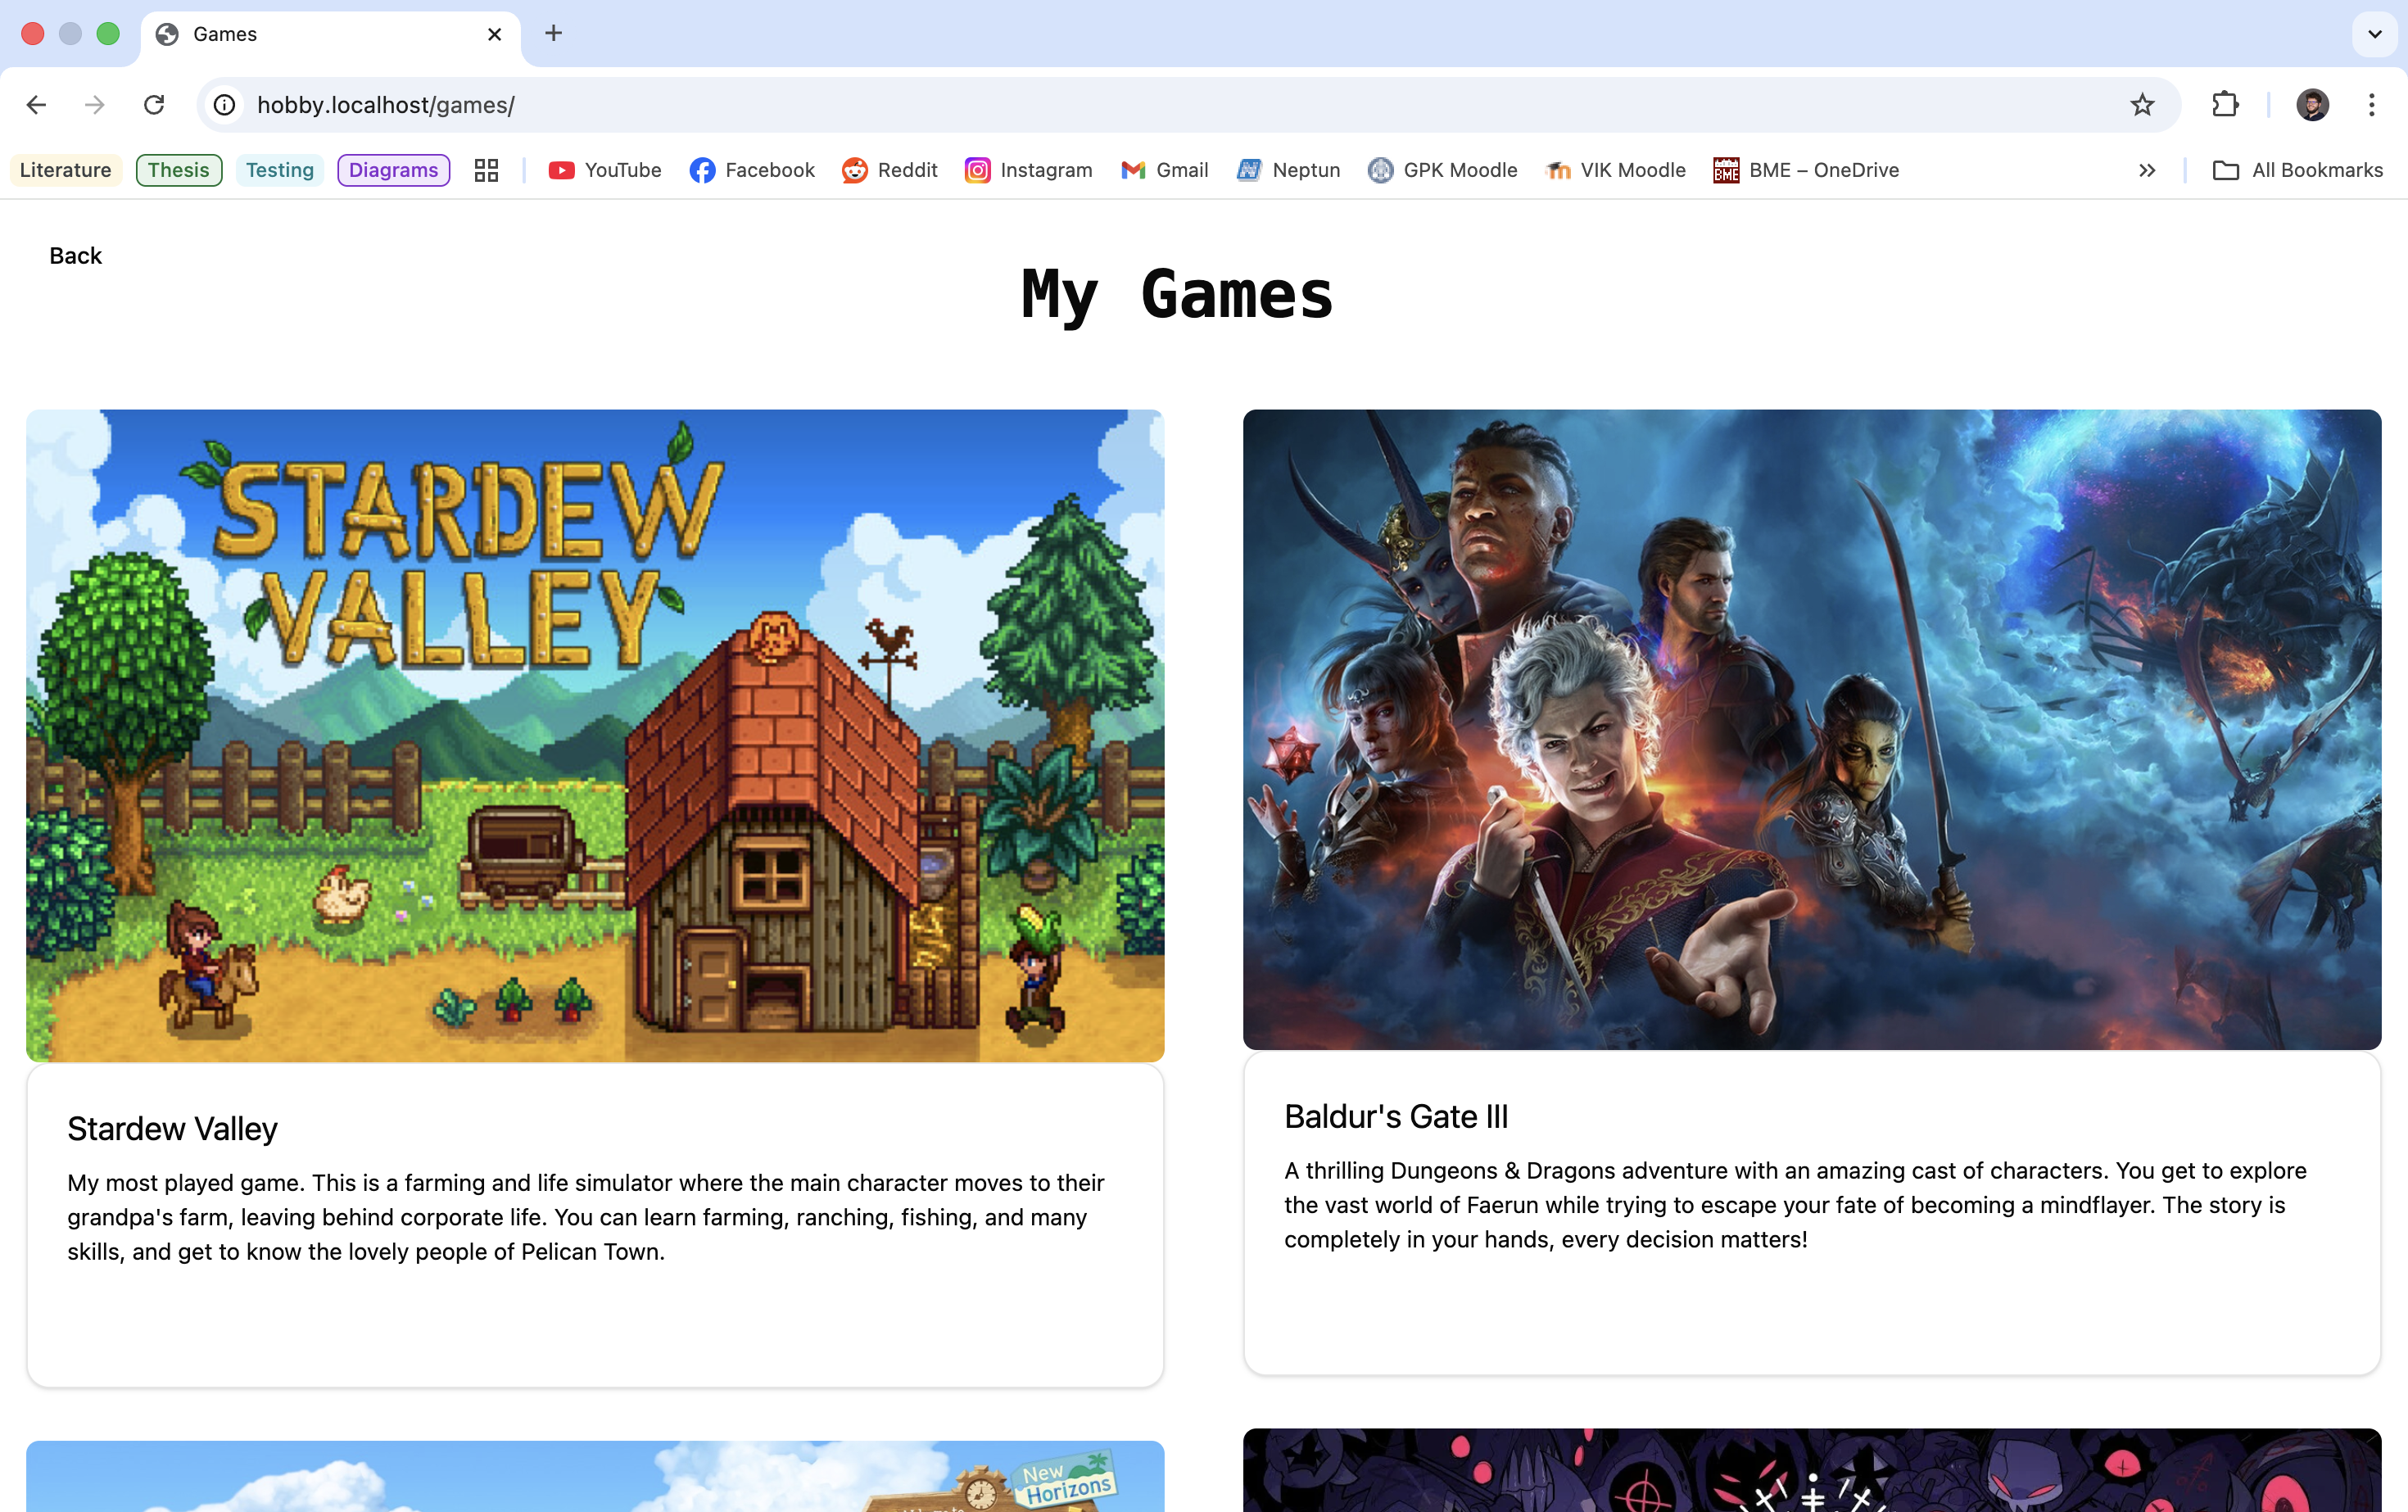
\includegraphics[width=\textwidth]{./figures/example/example-15.png}
    \caption{Games deployed}
    \label{subfig:example-published-games}
  \end{subfigure}
  \caption{Example site deployed}
  \label{fig:example-published}
\end{figure}

I will stop the example here, as it already showcases the main functionalities and capabilities of the application.
However, based on this short demo, it is easy to see how an end user may use the SaaS platform.
It can also be imagined that the user could easily follow these steps again, for example to edit this page further and redeploy the changes for others to see.